\documentclass[a4paper,11pt]{article}
\usepackage[utf8]{inputenc}
\usepackage[czech]{babel}
\usepackage{graphicx}
\usepackage{float}
\usepackage{hhline}
\usepackage[unicode]{hyperref}
\usepackage{amsmath}
\pagenumbering{arabic}

\begin{titlepage}
\title{Hledání nejkratších cest v grafu}
\date{\today}
\author{Tomáš Duda a Artemij Pozdňakov \\ dudatom2@fit.cvut.cz a pozdnart@fit.cvut.cz}
\end{titlepage}

\begin{document}

% Uvodni stranka
\maketitle
\newpage

% Obsah
\tableofcontents
\newpage

% Definici problému
% Popis sekvenčního algoritmu a jeho implementace
\section{Řešený problém a základní implementace}
\subsection{Definice problému}
Naším úkolem v rámci semestrálního projektu v předmětu BI-EIA je implementace a optimalizace dvou algoritmů pro hledání nejkratších cest v grafu. Vstupem programu je tedy graf zadaný výčtem hran a výstupem je délka nejkratší cesty pro každou dvojici uzlů.
\par
Pro řešení problému jsme implementovali dva algoritmy, první je Dijk\-strův, druhý Floyd-Warshallův. Jejich stručný popis a informace o základní implementaci jsou obsahem ná\-sle\-dujících částí.

\subsection{Dijkstrův algoritmus}
Dijkstrův algoritmus funguje obdobně jako prohledávání do šířky, jenom místo obyčejné fronty používá prioritní frontu. Do té jsou před během algoritmu přesunuty všechny uzlu, počáteční z nulovou, zbylé s $\infty$ vzdáleností. Poté se až do vyprázdnění fronty vybírá nejbližší uzel a pro všechny jeho sousedy se vyzkouší, zda byla nalezena zkracující cesta (relaxace). 
\par
Běžná verze Dijkstrova algoritmu je určena pro hledání nejkratších cest z jednoho uzlu do všech ostatních, proto ho musíme v našem řešení volat $|V|$-krát, tedy z každého uzlu. Asymptotická složitost Dijkstrova algoritmu závisí na dvou faktorech. Jednak jde o vnitřní reprezentaci grafu (seznam uzlů a jejich sousedů nebo matice sousednosti) a dále o způsob implementace prioritní fronty, kterou algoritmus využívá.
\par
V rámci snahy o kompromis mezi rozumnou rychlostí a dostatečnou možností kód následně optimalizovat jsme použili kombinaci reprezentace grafu seznamem sousedů a prioritní fronty řešené pomocí binární haldy. Tato kombinace má při hledání nejkratších cest mezi všemi dvojicemi uzlů asymptotickou složitost $\mathcal{O}(|V|(|E|+|V|)\log{|V|})$, kde V je množina uzlů a E je množina hran.

\subsection{Floyd-Warshallův algoritmus}
Floyd-Warshallův algoritmus hledá nejkratší cesty metodou postupné konstrukce. Skládá se ze tří do sebe vnořených cyklů, které iterují přes všechny uzly grafu. Vnější cyklus určuje prostředníka, přes které se algoritmus právě snaží nalézt zlepšující cestu, dva vnitřní cykly poté určují dvojici koncových uzlů.
Jako vnitřní reprezentace grafu je použita matice sousednosti, která je postupem algoritmu přepsaná na výslednou distanční matici. Asymptotická složitost Floyd-Warshallova algoritmu je $\mathcal{O}(|V|^3)$.

\subsection{Porovnání algoritmů}
Pro řídké grafy ($|E|\sim|V|$) má Dijkstrův algoritmus (s použitím binární haldy) nižší teoretickou složitost než Floyd-Warshallův. Dá se však očekávat, že při reálném použití u grafů, které jsme schopni v rozumném čase na poskytnutém HW upočítat (řádově tisíce uzlů), bude Floyd-Warshallův algoritmus rychlejší, jelikož potřebuje vykonat v nejvnitřnějším cyklu mnohem méně operací než Dijkstrův.

\subsection{Popis souborů}
\begin{itemize}
 \item \textbf{main.cpp} obsahuje zpracování argumentů z příkazové řádky a volání algoritmů.
 \item \textbf{mygraph.cpp} obsahuje třídu MyGraph, která jednak slouží pro vni\-třní reprezentaci grafu (podporuje jak matici sousednosti tak i reprezentaci pomocí seznamů uzlů a jejich sousedů). Dále realizuje zpracování vstupního grafu ze souboru.
 \item \textbf{node.cpp} a \textbf{edge.cpp} obsahují pomocné třídy pro uložení uzlu nebo hrany v grafu.
 \item \textbf{floydwarshall.cpp} implementuje Floyd-Warshallův algoritmus.
 \item \textbf{dijkstra.cpp} implementuje Dijkstrův algoritmus.
 \item \textbf{binary\_heap.cpp} poskytuje prioritní frontu přes binární haldu.
 \item \textbf{exception.cpp} definuje výjimku, která je použita při spuštění programu s chybnými argumenty.
\end{itemize}




% Popis případných úprav algoritmu a jeho implementace, včetně volby datových struktur
% Tabulkově a případně graficky zpracované naměřené hodnoty časové složitosti měřených instancí běhu programu s popisem instancí dat, přepočet výkonnosti programu na MIPS nebo MFlops.
% Analýza a hodnocení vlastností dané implementace programu.
\section{Optimalizovaná verze sekvenčního algoritmu}
Následující kapitola popisuje optimalizace provedené v sekvenčních verzích implementace a následné výsledky meření různých verzí.

\subsection{Dijkstrův algoritmus}
Jelikož nebylo Dijkstrův algoritmus možné optimalizovat klasickými metodami (vysoká datová provázanost, nemožnost rozbalit vnitřní cyklus kvůli komplikované datové struktuře), pokusili jsme se řešení optimalizovat více jinými způsoby. 
\par
\subsubsection{Úprava algoritmu}
Prvním byla výměna původně použité prioritní fronty z STL za vlastní implementaci, která navíc podporuje operaci decreaseKey a tudíž není po\-třeba u každého uzlu vyňatého z fronty testovat, zda je jeho hodnota klíče aktuální (zkrátka není nutné používat reinserting).
\subsubsection{Přepínače gcc}
Druhý pokus o optimalizaci proběhnul pomocí použití různých přepínačů při kompilaci v gcc.
\begin{itemize}
 \item \textbf{-O3} - zapnutí plných optimalizací cílového kódu.
 \item \textbf{-mffast-math} - zrychlené vyhodnocení matematických výrazů.
 \item \textbf{-msse4.2} - zapnutí vektorových instrukcí.
 \item \textbf{-mfpmath=sse} - použití SSE instrukcí místo klasických FP.
 \item \textbf{-msseregparm} - předávání FP dat přes SSE registry.
 \item \textbf{-mpc32} - zaokrouhlení FP výpočtů.
\end{itemize}
 Naopak testované, ale nakonec nepoužité zůstaly (neměly pozitivní vliv na rychlost): 
\begin{itemize}
 \item \textbf{-march=opteron} i \textbf{-march=barcelona}  - využití všech instrukcí na cílovém procesoru.
 \item \textbf{-regparm1..3} - jejich použití vyvalávalo na Staru segfault.
\end{itemize}
\subsubsection{Profiling}
V rámci profilingu jsme měřili čas strávený v jednotlivých řádkách kódu. Jako velmi neefektivní se ukázaly být vectory a iterátory z STL, které jsme nahradili obyčejným polem. Dále jsme zkusili odbourat zapouzdření v datových strukturách reprezentující graf, pomocí výčtu sousedů. Poslední úpravou, kterou se povedlo zlepšit čas běhu, bylo důsledné předpočítání všech položek (vzdáleností a indexů) před operací relaxace (v nejvnitřnějším cyklu Dijk\-strova algoritmu).
\par
Po všech úpravách profiler ukazuje, že přes 80 \% veškerého času tráví program přístupem do pole, ve kterém jsou uloženy aktuální vzdálenosti. To už se nám nepodařilo vylepšit. Přístup do tohoto pole není sekvenční (získáváme z něj vzdálenosti sousedů uzlu, který je aktuálně vytažen z prioritní fronty, tyto vzdálenosti mohou být na libovolném místě), a proto nemůžeme data z toho pole nějak "předpřipravit" před samotným výpočtem.

\subsection{Floyd-Warshallův algoritmus}
Byl použit loop-blocking pro lepší využití cache. Algoritmus se tím zrychlil až o polovinu. Testováním nám vyšla optimální hodnota parametru Bf (block factor) 32. Algoritmus ma pro každý blok (t,t) 3 fáze. Nejprve se spočítá samotný blok, poté bloky, které jsou ve stejném řádku nebo sloupci a nakonec všechny ostatní bloky. Dále je použit loop unrolling a vektorizaze, ta ale nemela moc velky efekt. Byly pouzity intrinsic instrukce, vektorizace pomoci kompilatoru se nezdarila.

\subsubsection{Přepínače gcc}
Implementace Floyd-Warshallova algoritmu poskytovala největší výkon při kompilaci s těmito přepínači:
\begin{itemize}
 \item \textbf{-O3} - zapnutí plných optimalizací cílového kódu.
 \item \textbf{-mffast-math} - zrychlené vyhodnocení matematických výrazů.
\end{itemize}
Naopak přepínače, které měly negativní vliv na výkon:
\begin{itemize}
  \item Celkově vektorizace, tedy přepínače \textbf{-msse4.2}, \textbf{-mfpmath=sse} \\a \textbf{-msseregparm}.
\end{itemize}

\subsection{Popis testovacích instancí}
Výběr testovacích instancí pro testování a porovnání obou implementovaných algoritmů byl poměrně komplikovaný. Dijkstrův algoritmus je narozdíl od Floyd-Warhsallova citlivý na vstupní data, tudíž bylo nutné, aby se jednotlivé testovací grafy lišily nejenom v počtu uzlů, ale i v počtu hran. 
\par
Floyd-Warshallův algoritmus se navíc ukázal být o hodně výkonnějším, tudíž zatímco neoptimalizovaná implementace Dijkstrova algoritmu na nej\-větší instanci za 60 minut na testovacím serveru nedoběhla, Floyd-Warshall ji upočítal za 10 minut.
\par
Vybrali jsme tedy grafy o čtyřech různých velikostech, co do počtu uzlů (800, 1600, 2400 s 3200) a u každého z nich tři různé instance lišící se poštem hran. První z trojice je vždy řídký graf (obsahuje přibližně desetinu hran, co graf úplný), druhý obsahuje přibližně polovinu hran úplného grafu a třetí je hustý, obsahuje 90 \% hran úplného grafu.
\begin{table}[H]
  \begin{center}
      \begin{tabular}{|r|r|r|}
      \hline
      Název souboru 	& Počet uzlů  	& Počet hran  		\\ \hline
      graf800\_80  	& 800    	& 31521             	\\ \hline
      graf800\_400     	& 800    	& 160035        	\\ \hline
      graf800\_720  	& 800    	& 287590             	\\ \hline
      graf1600\_160    	& 1600    	& 128022          	\\ \hline
      graf1600\_800  	& 1600    	& 639663             	\\ \hline
      graf1600\_1400   	& 1600    	& 1151713          	\\ \hline
      graf2400\_240  	& 2400    	& 289420             	\\ \hline
      graf2400\_1200   	& 2400    	& 1439793          	\\ \hline
      graf2400\_2160  	& 2400    	& 2591136             	\\ \hline
      graf3200\_320    	& 3200    	& 513016          	\\ \hline
      graf3200\_1600  	& 3200    	& 2560196             	\\ \hline
      graf3200\_2880   	& 3200    	& 4608704          	\\ \hline
      \end{tabular}
  \caption{Vlastnosti grafů, na kterých byly testovány sekvenční implementace algoritmů.}
  \label{tab:instance}
  \end{center}
\end{table}


\subsection{Měření a porovnání výkonosti různých sekvenčních verzí}
V následující části jsou uvedeny výsledky meření jednotlivých typů implementací. Údaje jsou uváděny v MFPLOPS. Zatímco i Floyd-Warshallova algoritmu můžeme počítat s~$2|V|^3$ operací v plovoucí čárce na jeden běh, u Dijkstrova algoritmu je situace o trochu komplikovanější, protože počet operací v FP závisí na podobě vstupního grafu a odhady pomocí složitosti nebyly příliš přesné. Změřili jsme tedy počet FP operací pro jednotlivé testovací instance.
\begin{table}[H]
  \begin{center}
      \begin{tabular}{|r|r|}
      \hline
      Název souboru 	& FP operací  	\\ \hline
      graf800\_80  	& 115,283 M            		\\ \hline
      graf800\_400     	& 524,098 M    		     	\\ \hline
      graf800\_720  	& 932,637 M    	            	\\ \hline
      graf1600\_160    	& 879,441 M    	        	\\ \hline
      graf1600\_800  	& 4,139 G    	           	\\ \hline
      graf1600\_1400   	& 7,414 G    	         	\\ \hline
      graf2400\_240  	& 2,912 G    	          	\\ \hline
      graf2400\_1200   	& 13,929 G    	         	\\ \hline
      graf2400\_2160  	& 24,956 G    	            	\\ \hline
      graf3200\_320    	& 6,800 G             		\\ \hline
      graf3200\_1600  	& 32,963 G    	            	\\ \hline
      graf3200\_2880   	& 59,136 G    	         	\\ \hline
      \end{tabular}
  \caption{Počet FP operací potřebných k běhu Dijkstrova algoritmu pro jednotlivé instance.}
  \label{tab:fp_operace}
  \end{center}
\end{table}

\subsubsection{Měření Dijkstrova algoritmu}
V následující tabulce jsou naměřené hodnoty pro Dijkstrův algoritmus. Mě\-ře\-na byla jednak verze, která využívá prioritní frontu z STL, poté verze používající prioritní frontu s podporou operace decreaseKey, třetí verze byla kompilovaná s pře\-pí\-načem -O3, ve čtvrté verzi byly použity další pře\-pí\-nače vypsané v sekci Optimalizovaná verze sekvenčních algoritmů. Nakonec jsou uvedeny hodnoty měření pro kód po profilingu.
\par

Z měření jde vypozorovat několik souvislostí:
\begin{itemize}
 \item Největší vliv na výkon mělo profilování kódu, kde byly odstraněny některé nadbytečné přístupy do paměti. Nicméně program i tak tráví prací s pamětí mnohonásobně více času, než samotnými výpočty. To je ale dáno potřebnou složitější datovou strukturou.
 \item Změna prioritní fronty z STL implementace na vlastní implementaci program mírně zrychlila.
 \item Při použití více přepínačů (než -O3) program pro většinu instancí zrychlí, ale výkony jsou mnohem méně stabilní.
\end{itemize}
\begin{table}[H]
  \begin{center}
      \begin{tabular}{|r|r|r|r|r|r|}
      \hline
      Instance  	& STL	  & BH    & -O3	 & k. opt  & prof  \\ \hline
      graf800\_80  	& 11,9  & 20,8	  & 50,8 & 50,1    & 96,0  \\ \hline
      graf800\_400     	& 15,5  & 16,7 	  & 25,5 & 27,9	   & 55,0  \\ \hline
      graf800\_720  	& 13,0  & 15,9 	  & 28,9 & 32,7	   & 52,0  \\ \hline
      graf1600\_160    	& 12,3  & 16,9 	  & 28,4 & 27,5	   & 47,5  \\ \hline
      graf1600\_800  	& 14,4  & 15,6 	  & 26,6 & 30,0	   & 50,9  \\ \hline
      graf1600\_1400   	& 14,8  & 16,4 	  & 25,4 & 29,7	   & 52,1  \\ \hline
      graf2400\_240  	& 11,8  & 15,3	  & 25,1 & 23,2    & 35,8  \\ \hline
      graf2400\_1200   	& 14,2  & 15,4	  & 24,8 & 24,9    & 51,6  \\ \hline
      graf2400\_2160  	& 14,8  & 12,6	  & 25,1 & 26,9    & 49,5  \\ \hline
      graf3200\_320    	& 12,3  & 12,7	  & 23,7 & 24,9    & 39,0  \\ \hline
      graf3200\_1600  	& 14,3  & 14,9	  & 25,0 & 28,0    & 52,7  \\ \hline
      graf3200\_2880   	& x    	& x 	  & 25,1 & 27,1    & 50,0  \\ \hline
      \end{tabular}
  \caption{Naměřené výsledky pro Dijkstrův algoritmus. Hodnoty jsou v~MFLOPS. Políčka, ve kterých je uvedeno x značí, že pro ně algoritmus nedokázal doběhnout ve stanoveném limitu 60 minut.}
  \label{tab:dijkstra1}
  \end{center}
\end{table}


\subsubsection{Měření Floyd-Warshallova algoritmu}
Ve prvním sloupci NoOpt jsou výsledky meření výchozího programu bez použití žádných optimalizací. V dalších je kompilace se základní optimalizací kompilátoru -O3. Další měřená verze je po transformacích kódu popsaných v kapitole 2.2.
\begin{table}[H]
  \begin{center}
      \begin{tabular}{|r|r|r|r|r|}
      \hline
      Instance  	& NoOpt	    & -O3     & Transf	   \\ \hline
      graf800\_80  	& 129,0     & 975,2   & 1177,0     \\ \hline
      graf800\_400     	& 130,4     & 890,4   & 1248,7     \\ \hline
      graf800\_720  	& 129,3     & 1402,7  & 1190,7     \\ \hline
      graf1600\_160    	& 125,2     & 686,7   & 1233,7     \\ \hline
      graf1600\_800  	& 125,3     & 688,4   & 1180,4 	    \\ \hline
      graf1600\_1400   	& 125,2     & 680,9   & 1177,0 	    \\ \hline
      graf2400\_240  	& 126,0     & 670,7   & 1201,0           \\ \hline
      graf2400\_1200   	& 126,1     & 671,0   & 1209,9           \\ \hline
      graf2400\_2160  	& 126,4     & 670,0   & 1326,0           \\ \hline
      graf3200\_320    	& 125,8     & 665,6   & 1276,2           \\ \hline
      graf3200\_1600  	& 126,0     & 663,6   & 1303,2           \\ \hline
      graf3200\_2880   	& 125,9     & 662,9   & 1347,9           \\ \hline
      \end{tabular}
  \caption{Naměřené výsledky pro Floyd-Warshallův algoritmus. Hodnoty jsou v~MFLOPS.}
  \label{tab:fw2}
  \end{center}
\end{table}



% Popis případných úprav algoritmu a jeho implementace, včetně volby datových struktur
% Tabulkově a případně graficky zpracované naměřené hodnoty časové složitosti měřených instancí běhu programu s popisem instancí dat, přepočet výkonnosti programu na MIPS nebo MFlops.
% Analýza a hodnocení vlastností dané implementace programu.
\section{Vícevláknová implementace}
Následující kapitoly se zabývá vícevláknovou implementací Dijkstrova a Floyd-Warshallova algoritmu pomocí knihovny OpenMP. Zvlášť pro každý algoritmus jsou zde popsány provedené úpravy a měření zrychlení.
\subsection{Dijkstrův algoritmus}
U paralelizace Dijkstrova algoritmu s nabízely dvě možnosti. První bylo přepsání Dijkstrova algoritmu do paralelní verze. Tuto cestu jsme nezvolili, protože by nešlo jednoduše zrychlení oproti jednovláknové verzi a navíc by samotná paralelizace v OpenMP byla komplikovaná.
\par
Druhá možnost, kterou jsme zvolili, je mnohem jednodušší. Jelikož Dijk\-strův algoritmus při výpočtu vzdáleností mezi všemi dvojicemi uzlů voláme n-krát, základní jednotkou práce bude najití nejkratších cest právě pro jeden jeden počáteční uzel.
\par
Samotná implementace probíhala ve dvou krocích. Prvním krokem bylo přepsání algoritmu do jediné metody, aby byly všechny používané proměnné viditelné pro OpenMP (v původní implementaci byl problém například s třídními proměnnými).
\par
Druhým krokem bylo dopsání direktiv pro OpenMP a doplnění mechanismu pro složení výsledné distanční matice z dílčích výsledků jednotlivých vláken. Při implementaci tohoto mechanismu se ukázalo, že se vyplatí výsledek skládat postupně (za cenu malé kritické sekce v cyklu), než alokovat pro každé vlákno speciální distanční matice a výsledek složit po doběhnutí posledního vlákna (nejspíš kvůli méně efektivní práci s cache pamětí a komplikovanější adresaci v rámci jednotlivých distančních matic). 
\par
Ladění paralelní verze spočívalo ve volbě nejlepší strategie pro rozdělení iterací mezi jednotlivá vlákna. Měření jednotlivých možností je obsahem následující podkapitoly.

\subsubsection{Měření}
OpenMP nabízí pro paralelizaci cyklů tři strategie - static, dynamic a guided. Jelikož je délka běhu Dijkstrova algoritmu závislá na vstupním grafu a zvoleném počátečním uzlu, předpokládali jsme, že se vyplatí dynamické plánování za cenu větší režie.
\par
Naměřené výsledky pro různé strategie, velikosti jednotlivých částí práce a různě husté vstupní grafy jsou zobrazeny v tabulce a grafu níže. Jednotlivé sloupečky tabulek odpovídají nastavené velikosti práce pro jedno vlákno. První řádek je pro řídký graf (desetina hran úplného grafu), druhý pro středně hustý (polovina hran úplného grafu) a třetí pro skoro úplný graf (děvět desetin hran úplného grafu. Údaje jsou zde v sekundách. Program byl spouštěn na 12 vláknech.

\begin{table}[H]
  \begin{center}
      \begin{tabular}{|r|r|r|r|r|r|r|}
      \hline
      
      Instance  	& 1	    & 2		& 4	& 8	& 16 	& 32	   \\ \hline
      graf3200\_320	& 26,76 & 27,57 & 10,25	&28,01 	&28,67 	&67,45 \\ \hline
      graf3200\_1600	& 124,04 & 129,12 & 124,21 & 132,15 & 129,23 &235,45 \\ \hline
       graf3200\_2880	& 217,31 & 223,74 & 219,28 & 223,38 & 219,68 & 410,38 \\ \hline

      \end{tabular}
  \caption{Strategie static.}
  \label{tab:static}
  \end{center}
\end{table}

\begin{table}[H]
  \begin{center}
      \begin{tabular}{|r|r|r|r|r|r|r|}
      \hline
      
      Instance  	& 1	    & 2		& 4	& 8	& 16 	& 32	   \\ \hline
      graf3200\_320	& 27,08 & 26,93 & 26,96 & 26,45 & 26,03 & 26,78 \\ \hline
      graf3200\_1600	& 120,10 & 126,1 & 121,33 & 128,91 & 123,384 & 130,07 \\ \hline
      graf3200\_2880	& 209,57 & 220,11 & 212,00 & 220,14 & 212,261 & 221,65 \\ \hline
      
      \end{tabular}
  \caption{Strategie guided.}
  \label{tab:guided}
  \end{center}
\end{table}

\begin{table}[H]
  \begin{center}
      \begin{tabular}{|r|r|r|r|r|r|r|}
      \hline
      
      Instance  	& 1	    & 2		& 4	& 8	& 16 	& 32	   \\ \hline
      graf3200\_320	& 25,57 & 25,63 & 26,47 & 25,86 & 26,62 & 26,05 \\ \hline
      graf3200\_1600	& 119,96 & 120,48 & 127,68 & 120,84 & 129,56 & 125,51\\ \hline
      graf3200\_2880	& 208,51 & 208,85 & 221,18 & 209,72 & 223,82 & 213,66 \\ \hline
      
      \end{tabular}
  \caption{Strategie dynamic.}
  \label{tab:dynamic}
  \end{center}
\end{table}

\begin{figure}[H]
  \begin{center}
    \includegraphics[scale=0.9]{dijk.png}
  \end{center}
  \caption{Porovnání jednotlivých strategií pro různě husté grafy. Modře jsou vyneseny výsledky strategie guided, zeleně strategie dynamic a oranžově static.}\label{graf:fig7}
\end{figure}

Z výsledků je vidět, že mezi strategiemi (s výjimkou static pro větší velikost) je relativně malý rozdíl. Jako nejefektivnější se tedy těsně ukázala být strategie dynamic s velikostí 1.
\par
Pro úplnost v tabulce níže uvádím přepočet konečných výsledků do MFLOPS a jejich porovnání s předchozími verzemi implementace.

\begin{table}[H]
  \begin{center}
      \begin{tabular}{|r|r|r|r|}
      \hline
      Instance  	& 1vl. neopt.   & 1vl. opt. & paralelní\\ \hline
      graf800\_80  	& 11,9  & 96,0 & 129,5 \\ \hline
      graf800\_400     	& 15,5  & 55,0 & 415,9 \\ \hline
      graf800\_720  	& 13,0  & 52,0 & 330,7 \\ \hline
      graf1600\_160    	& 12,3  & 47,5 & 420,8\\ \hline
      graf1600\_800  	& 14,4  & 50,9 & 277,0 \\ \hline
      graf1600\_1400   	& 14,8  & 52,1 & 284,3 \\ \hline
      graf2400\_240  	& 11,8  & 35,8 & 298,6 \\ \hline
      graf2400\_1200   	& 14,2  & 51,6 & 269,5 \\ \hline
      graf2400\_2160  	& 14,8  & 49,5 & 278,8 \\ \hline
      graf3200\_320    	& 12,3  & 39,0 & 265,9 \\ \hline
      graf3200\_1600  	& 14,3  & 52,7 & 274,8 \\ \hline
      graf3200\_2880   	& x    	& 50,0 & 283,6 \\ \hline
      \textbf{Průměr}	& 12,4  & 52,8 & 294,3 \\ \hline
      \end{tabular}
  \caption{Naměřené výsledky pro Dijkstrův algoritmus. Hodnoty jsou v~MFLOPS. Políčka, ve kterých je uvedeno x značí, že pro ně algoritmus nedokázal doběhnout ve stanoveném limitu 60 minut. V prvním sloupci jsou výsledky pro jednovláknovou implementaci bez optimalizací, druhý sloupeček pro jednovláknovou optimalizovanou implementaci a poslední pro finální paralelní verzi (12 vláken).}
  \label{tab:dijkstra2}
  \end{center}
\end{table}
Z měření je vidět téměř 6násobné zrychlení oproti jednovláknové implementaci. Jde tedy přibližně o poloviční využití teoretické výpočetní síly všech 12 jader procesoru.

\subsection{Floyd-Warshallův algoritmus}
Kvuli loop-blockingu se se algoritmus paralelizoval snadno. Staci dodrzet, aby se nejprve spocitaly samotne bloky, pote bloky na stejnem radku a sloupci a pote zbytek. Paralelizoval se kazdy z techto cyklu. Vlakna byla vytvorena hned na zacatku, kvuli zmenseni rezie cyklu. Jine planovani vlaken nez static by nemelo mit pozitivni vliv na rychlost algoritmu, protoze jsou bloky stejne velke.

\begin{figure}[H]
  \begin{center}
    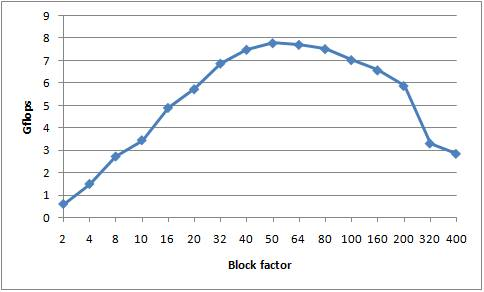
\includegraphics[scale=0.7]{bf.jpg}
  \end{center}
  \caption{Porovnani jednotlivych velikosti BF.}\label{graf:fig8}
\end{figure}

Velikost bloku BF jsme zvolili 50.
\subsubsection{Měření}
Pro porovnani vykonnosti je tu sequencni neoptimalizovana verze, optimalizovana verze pouze pomoci kompilatoru, celkove optimalizovana a paralelni verze.

\begin{table}[H]
  \begin{center}
      \begin{tabular}{|r|r|r|r|r|}
      \hline
      Instance  	& NoOpt	    & -O3     & SeqOpt	& Paralelni	\\ \hline
      graf800\_80  	& 129,0     & 975,2   & 1177,0	& 5779,8     	\\ \hline
      graf800\_400     	& 130,4     & 890,4   & 1248,7	& 5779,8     	\\ \hline
      graf800\_720  	& 129,3     & 1402,7  & 1190,7	& 5779,8     	\\ \hline
      graf1600\_160    	& 125,2     & 686,7   & 1233,7	& 7204,3     	\\ \hline
      graf1600\_800  	& 125,3     & 688,4   & 1180,4	& 7183,9    	\\ \hline
      graf1600\_1400   	& 125,2     & 680,9   & 1177,0	& 7335,9    	\\ \hline
      graf2400\_240  	& 126,0     & 670,7   & 1201,0	& 8104,8       	\\ \hline
      graf2400\_1200   	& 126,1     & 671,0   & 1209,9	& 8097,2      	\\ \hline
      graf2400\_2160  	& 126,4     & 670,0   & 1326,0	& 8145,9       	\\ \hline
      graf3200\_320    	& 125,8     & 665,6   & 1276,2	& 8003,5       	\\ \hline
      graf3200\_1600  	& 126,0     & 663,6   & 1303,2	& 8041,5       	\\ \hline
      graf3200\_2880   	& 125,9     & 662,9   & 1347,9	& 8135,8       	\\ \hline
      \end{tabular}
  \caption{Naměřené výsledky pro Floyd-Warshallův algoritmus. Hodnoty jsou v~MFLOPS.}
  \label{tab:fw1}
  \end{center}
\end{table}
Z měření je vidět vice nez sestinasobné zrychlení oproti jednovláknové implementaci.

\newpage

% Závěr
\section{Závěr}
V rámci semestrální práce jsme implementovali, optimalizovali a paralelizovali algoritmy pro hledání nejkratších cest v grafu - Dijkstrův a Floyd-Warshallův. Zrychlení u obou algoritmů mezi první a finální verzí bylo více jak dvacetinásobné.
\par
Prokázal se předpoklad, že Floyd-Warshallův algoritmus bude rychlejší než Dijkstrův. Je tomu tak zejména díky jeho jednoduchosti - pracuje s mnohem méně komplikovanými datovými strukturami.


\newpage
\begin{thebibliography}{1}
  \bibitem[1]{Kolar} KOLÁŘ, Josef.
    \emph{Teoretická informatika}.
    Česká informatická společnost, Praha, 2004. 205s.
  \bibitem[2]{FwBlock} LUND, Ben, SMITH, Justin W..
    \emph{A Multi-Stage CUDA Kernel for Floyd-Warshall}.
    [online]. Dostupné z: \url{http://arxiv.org/pdf/1001.4108.pdf}. [cit 11-18-2014]. 2010.
\end{thebibliography}

\end{document}

